\documentclass[12pt,oneside,a4paper]{article}
\usepackage{blindtext}
\usepackage{setspace}
\usepackage[left=1.5in, right=1in, top=1in, bottom=1in]{geometry}
\usepackage{graphicx} %TO include graphics in document
\usepackage{amssymb}
\usepackage{algorithm}% http://ctan.org/pkg/algorithms
\usepackage{algpseudocode}% http://ctan.org/pkg/algorithmicx
\usepackage{url} %for including urls in References
\usepackage{cite}
\usepackage{pdfpages} % To include title page pdf

\begin{document}
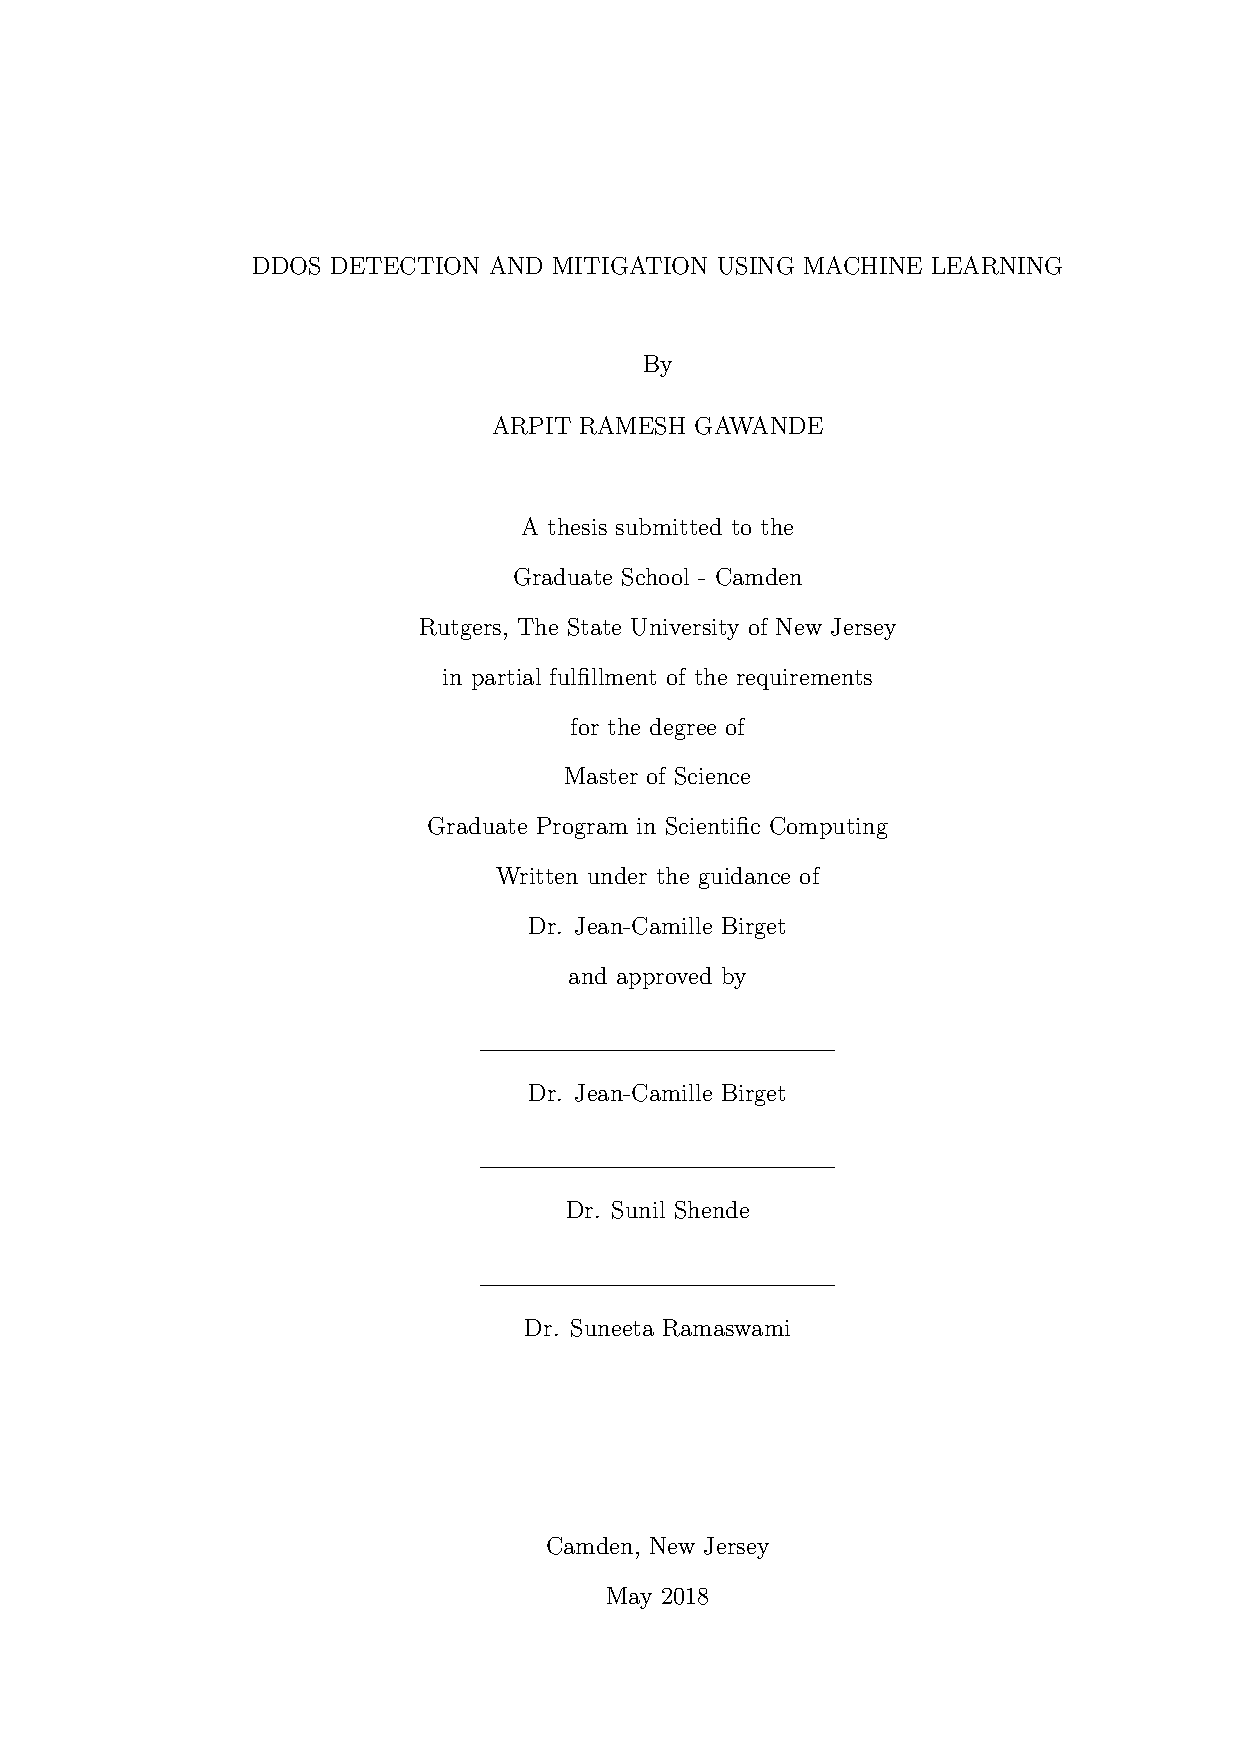
\includepdf{title}
\doublespacing
\renewcommand{\thepage}{\roman{page}}% Roman numerals for page counter
\setcounter{page}{2}% Start page number with 2
\tableofcontents
\newpage
%For page numbering at top right of the page
\pagestyle{myheadings}
\renewcommand{\thepage}{\arabic{page}}% Arabic numerals for page counter

\begin{abstract}
Distributed Denial of Service (DDoS) attacks are very common these days\cite{ddos-attack-news}. It is evident that the current industry solutions such as completely relying on Internet Service Provider(ISP) or setting up DDoS defense infrastructure are not sufficient in detecting and mitigating DDoS attacks, hence consistent research is needed. Most of the current industry solutions involve setting up a centralized expensive hardware system which can analyze the data packets \cite{network-data-packet} for probable DDoS attacks. Also each router provider has different protocols to communicate between the DDoS attack detection system and the router/networking devices, limiting the reach of DDoS detection systems. In this paper we are going to discuss a way to detect DDoS attack using machine learning tools at the routers instead of setting a centralized analysis system. Also we are proposing a standard communication architecture which can be used across all the networking devices for mitigating DDoS attacks.
\end{abstract}

\section{Existing Systems}

\subsection{What it DDoS attack}
Distributed Denial of Service (DDoS) attack is a way to jam a host network or its resources with a large number of data packets\footnote{Messages that are sent on the Internet are broken into shorter messages for transmission. These short messages are called packets. Term coined by Donald Watts Davies.} or connections, so that the host becomes disabled. There are different types of DDoS attacks such as :
1. Volume based, e.g. SYN Flood Attacks, in which the victim is flooded with a hight volume of packets or connections.
2. Application based, in which an application such as DNS, VOIP or HTTP are attacked.
3. Low rate DDoS attacks, in which the attacker exploits a vulnerability in the application design, e.g. Slowloris.
\cite{DDoS-attacks}

\subsection{Challenges in dealing with DDoS attacks}
The real challenge in detecting and defending against DDoS attack is because of its dynamic nature. The source\footnote{It is a system/device on the Internet that has an IP address and which is involved in DDoS attack} is not a single node or a system on the Internet but there can be many systems participating in DDoS attack, and often these systems are distributed over different regions of the Internet. Also the source of the packet is often spoofed\footnote{spoofing is the way to change the source IP address of the message. This is a known issue in the protocol itself not in the implementation}\cite{ip-spoofing}, which makes harder to know the actual IP address of the system from where attack is originated because original attack source is changed in spoofed data packet. In addition to that, many times the source system itself is not aware that it is compromised and it is being used as a bot\cite{bot} by an attacker to launch DDoS attack.

Because the source address can not be a reliable way to know the attack source, detecting and mitigating attack at the destination\footnote{System under DDoS attack} is not very useful. Destination may know that the attack is happening but to stop it happening it will have to block all the incoming traffic including the legitimate traffic. To avoid this, many network device producing companies such as Cisco, Netgear have come up with some solutions. Many of the solutions provided by those giant or the research that is done in this field has been focusing on collecting network traffic flow information\cite{network-traffic-flow} at routers(gateways). A flow consist of a number of Internet packets captured during a fixed time interval. Router send that flow information to the central system for analysis. Central system is a hardware and software infrastructure which is capable of processing and analyzing large flow information.\par

Some of the major protocols which are widely used for flow collection and analysis are, Internet Protocol Flow Information Export (IPFIX) protocol created by the Internet Engineering Task Force (IETF), Ciscos NetFlow\cite{cisco-netflow} and Sflow(Sampled flow)\cite{sflow}. These protocols have defined standard way to export the flow information from router and similar devices. All these flow monitoring protocols gather information and send the consolidated flow information to the centralized server where user can login and perform functions; such as Security Monitoring, Bandwidth monitoring, Resource Management, Traffic Analysis, Performance Management etc. On such systems, there are some modules which are specifically used for anomaly/DDoS detection.\par

E.g. Cisco netflow has flow exporter, collector and analysis modules. Flow exporter modules are installed on routers. The routers which are having flow exporter modules, send flow information to collector module installed on the server. Along with the collector module server also has analysis module which can be used to detect different patterns in the flow.\par

These technologies scales well and can be sufficient to indicate trends in network traffic but they have limitations. 1) They are not cross platform, e.g. router with Sflow protocol can not work with Cisco routers. 2) They involve setting up expensive hardware which acts as collector server. 3) Source address is used for flow analysis which is not reliable due to IP spoofing in the case of of DDoS attack.\par

Now we know that the router based flow analysis can be useful for anomaly detection but it has limitations. We don't want to set up expensive hardware, we want to have a protocol or a system which is compatible with other routers. Also we don't want source IP address for detection analysis. So if we can come up with a way by which we can detect anomaly in the traffic at the router and create a communication protocol between the router and the destination server or network, then router and network can take better decisions on regulating the packet flow. If we use only the destination IP address for analysis, then we will be more efficient in detecting and mitigating DDoS attacks.

\section{DDoS Detection and Mitigation}

DDoS attacks can be detected by checking if there is any anomalous behavior in the network traffic, such as, sudden increase in the number of packets going to a destination. This can be done at server by observing all the incoming traffic or it can be done by observing all the out going traffic at ISP or at every router. Attack can be mitigated if the anomalous packet are blocked reaching their destination.

\section{Network Functioning}

\subsection{Point of knowledge}
A switch creates a network and router connects those networks. A router links computers to the Internet through other routers. Routers are the backbone of the network who helps to forward packet from one point to other point on the Internet. Every packet traveling on the Internet has to go through a router\cite{router-switch}. Router knows where the packet is destine hence it could serve as first point of knowledge about the change in the flow information for a destine network. Each router has interfaces to which hosts or other network are connected. So router is aware to whom it is connected. Router uses protocol to communicate between other networking devices and by that it gathers knowledge about other networks or routers on the Internet. ICMP\cite{icmp} is one of the most frequently use protocol by routers to communicate.\par

\begin{figure}[H]
\centering
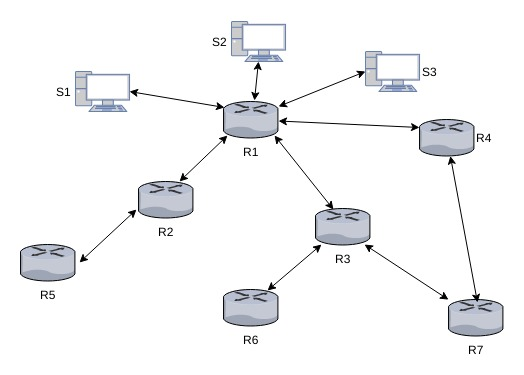
\includegraphics[width=0.70\textwidth]{routers.jpg}
\caption{Network Example} \label{fig:routers}
\end{figure}


Let's illustrate this using an example. In the above figure we can see that host S1, S2, S3 are connected to a router R1. Router R1 is connected to Internet through router R2, R3 and R4, thus every packet reaching to the system S2 is coming from either of these three routers. All three routers are located in different geographical region. Most of the websites are regional, either county, state or national (If we leave out few global websites) and hence they are mostly accessed from those region it is meant for. E.g. Rutgers University website is accessed mostly from the eastern region of United States and that too mostly from the New Jersey State or the Philadelphia region.\par
Using traceroute we can find out how many hops\footnote{hops are intermediate routers in the communication channel} away the destination is. Following is one of the captured traceroute for Rutgers University website.\par
%\vspace{5mm} % vertical space
\begin{figure}[H]
\centering
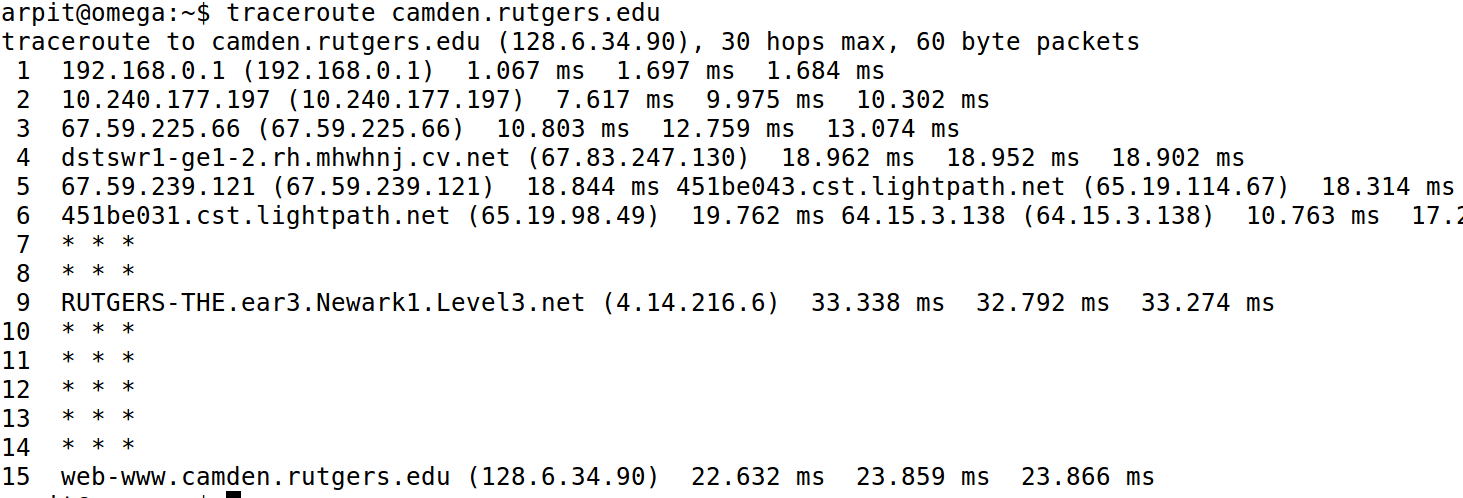
\includegraphics[width=0.90\textwidth]{TraceRoute.png}
\caption{Trace Route: All the routers in the path to destination} \label{fig:traceroute}
\end{figure}

We can see that the packet traverse through the 15 routers to reach to camden.rutgers.edu server. This trace route is taken from a location in the New Jersey State.\par

\section{Our Approach}

\subsection{Router as point of analysis}
From Figure \ref{fig:routers} and \ref{fig:traceroute} we know that routers are located at different geographical locations and also there are specific regions from which a given website/web server is accessed(except few). Some of the service providers such as  GeoIP or Google, can find out the location from where the traffic is coming in the network for a given website, but that is approximate based on the source IP. In the case of DDoS attack this information is unreliable, because the packet source address is often spoofed. This makes difficult to know the actual geographical location from which the packet has come, but routers through which that packet has traveled can provide their own geographical information. Such information can be useful to understand the path through which a packet has traveled and thus we can know the region from which the packet is originated.\par

In the normal scenario there is a consistency in which website is accessed from different geographical regions, and this consistency can be found by measuring the number of requests or packets traveled from a router to a destination server. This behavior of accessing different website from a router can be learned over the time. Thus finding this behavior in a flow\footnote{In this paper we will consider flow only in sense of destination address} at the router can form the basis of analysis in this paper. If there is a deviation from the learned behavior of accessing particular destination, then that change in behavior as well as router geographical region information can be communicated to the destination network. The destination network on receiving that information, can decide, whether it want the reporting router to discard or forward the traffic for it. This is a selective process in which traffic from only specific router is blocked while traffic from other routers remain unaffected\par

With the advance of electronic and the Internet of things, processing and storage capacity of the electronic devices has increased. Router is also not left behind, but storage capacity of router is always very less compared to server which collect flow data for network traffic analysis. If we use the learning techniques which don't need much storage then we don't have to store large chunk of packets on the router. Instead of storing data packets for longer time for analysis, we can learn from small number of packets and then discard packets once learning is done leaving behind only the learned information on the router. This is necessary because the number of entries on the Internet routing table has steadily grown. Now that the table has passed 500,000 routes\cite{routing-tablesize} so storing each and every flow information for these routes could be difficult.\par

\begin{figure}[H]
\centering
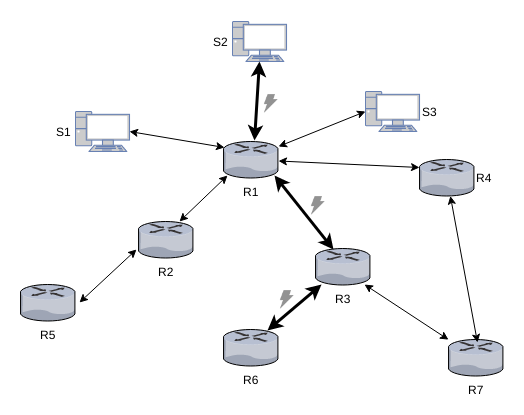
\includegraphics[width=0.70\textwidth]{attack_path.png}
\caption{DDoS Attack path} \label{fig:attackpath}
\end{figure}


In the above figure an attack is initiated from the region where router R6 is located and from router R6 data packets travel to the victim\footnote{Victim is a computer system which is under DDoS attack} system S2. Attack packets traveled through router R3 and R1 to reach system S2. If we can detect attack at router R6, then router R6 can discard all the packets heading towards system S2. In this process, only traffic from router R6 is affected but traffic from all other routers remain unaffected.

To achieve this, we will gather the flow information during a time window (e.g 300 sec) whose size will be fixed at the beginning. Thus a flow will contain all the packets traveled from a router to different destinations during a time span of 300 seconds. We can also combine such flows to form a new flow with bigger time windows. e.g. if we combine two flow of 300 seconds then we will have flow of 600 seconds. This flow information can be capture during particulate period or through out the day. Once we have flow information we can apply learning techniques on each flow iteratively to gain deeper knowledge about normal behavior of the flow. e.g. on average, how many packets of different protocols are destine for a given destination from a given router/region during a particular time of the day.

\begin{figure}[H]
\centering
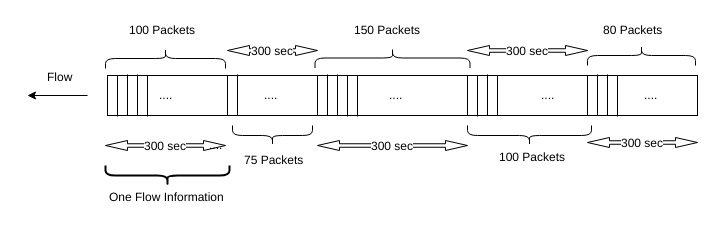
\includegraphics[width=0.90\textwidth]{Data_Flow_Capture.png}
\caption{300 second time segment correspond to a flow information. The number of packets can vary in a flow.} \label{fig:flow}
\end{figure}

\subsection{Analysis techniques to be implemented}
In the proposed system, each router will itself act as an analyzer. Each packet will be analyzed and flow statistic is created based on the destination IP address. Based on the statistic, clustering of destination IP address using input feature vector is done. Clustering is the process of examining a collection of “points,” and grouping the points into “clusters” according to some distance measure. The goal is to minimize the distance of the point in the cluster to other points in the same clusters.\cite{machine-learning}.

Once the clustering is learned, it will be used as a bench mark for all future flow. Router will constantly keep clustering destination IP address and if there is deviation in the normal traffic at router for any destination then that will affect the clustering and it will cause destination to be placed in different cluster. This change in the cluster for a given distention can be marked as change in the behavior of the traffic for that destination. Along with the cluster we will also use Novelty Detection algorithm to achieve more accurate result. This change in traffic behavior will be reported to destination network, which then decide on regulating the traffic coming to itself from the router which has send the information\par

\section{Implementation}

As discussed previously, there are different types of DDoS attacks, such as Volume based, Application based and also Low rate DDoS attacks. Among these different types of DDoS attacks, the volume based attacks are most common. In the volume based attack, victim is flooded with a high volume of Internet packets (TCP, UDP, HTTP or ICMP) make it unable to serve the requests.

For the demonstration of the suggested approach we are simulating a volumed based bot attack. Bots are the compromised computer systems, controlled by an attacker for launching an attack. They are not bounded by the geographical boundaries, so they can be anywhere in the Internet. Botnet(Network  of bots) are employed by an attacker to launch a DDoS attack. As we know that the Internet is connection of different computer system that communicate with each other, through different channels such as cables, satellite or radio device and these communication channels run throughout the glob; connecting different computer systems at different locations.

We are using Wireshark, an open source tool, for capturing Internet packets. Wireshark can capture all digital information received or sent through different devices such as Ethernet or wifi devices, which connects computer to the Internet. It also helps identify different protocol packets (e.g. TCP, UDP) within the wrapper packet created at Data Link Layer packet. Data Link Layer packet is a wrapper over all higher protocols such as TCP/UDP in OSI model.\par

\begin{figure}[H]
\centering
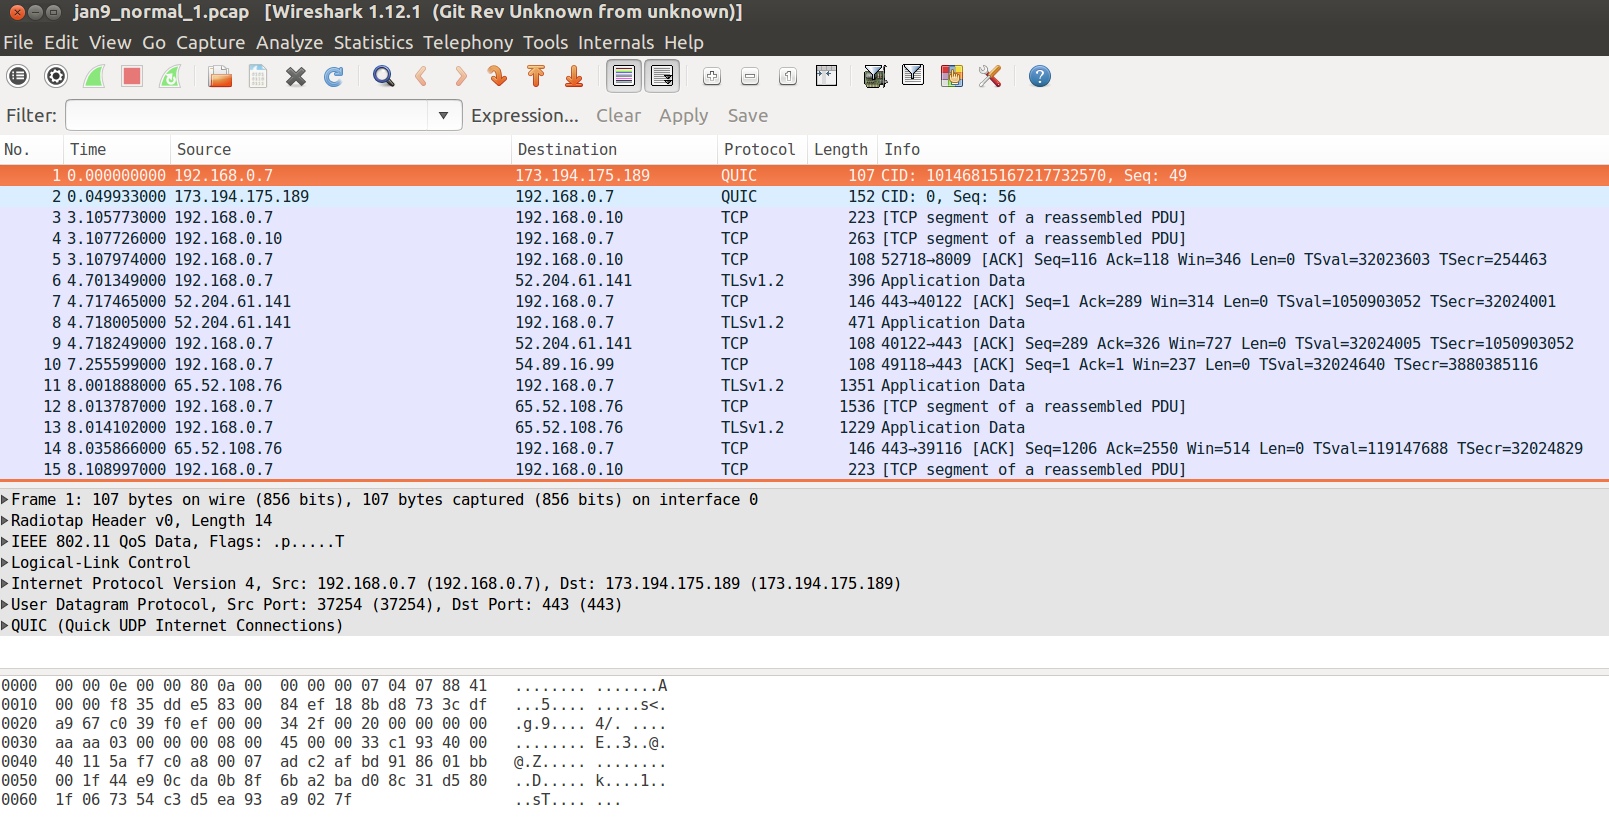
\includegraphics[width=0.90\textwidth]{Wireshark_Tools.png}
\caption{Wireshark Tool: snippet of captured packets} \label{fig:wireshark}
\end{figure}

To gather data for the demonstration, we have created a small network which has one router and couple of host machine. Each machine can be a victim of DDoS attack. We have installed Wireshark tool on one of the machine in the this network. For capturing traffic in the network we are using the Promiscuous mode of Wireshark. In Promiscuous mode, network interface can record not only the traffic that is intended to itself but all of the traffic on the network, so we can see all in out traffic in our setup network. This setup is similar to any router on the Internet which is connected with different routers and hosts.

\begin{figure}[H]
\centering
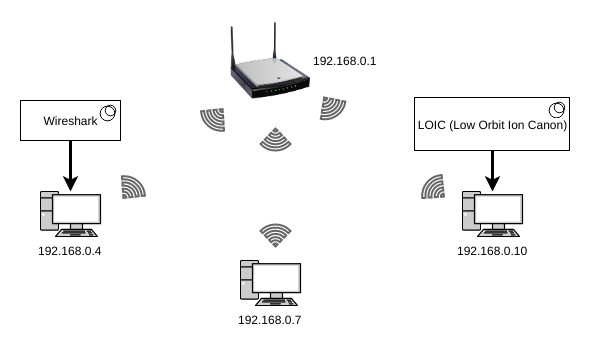
\includegraphics[width=0.90\textwidth]{demo_network.png}
\caption{Demo Network: for purpose of demonstration} \label{fig:demonetwork}
\end{figure}

To collect packets traveling in our network, we start the Wireshark tool. We let it run for a while and then we orchestrate a DDoS attack on one of the host (e.g. 192.168.0.7 in Figure \ref{fig:demonetwork}) in the network. This attack is engineered using the Low Orbit Ion Canon(LOIC) tool which is installed on one of the host (e.g. 192.168.0.10 in Figure \ref{fig:demonetwork}) in our network. LOIC is a free tool which is even used by attackers in the real world DDoS attacks. This tool allow us to launch TCP and UDP flood attack on any destination. In this paper we are analyzing the flow based TCP and UDP attack, which is one of the most common type of DDoS attacks.

In the LOIC tool we need to give IP address and the port number of the destination where we want to orchestrate attack while rest of the work is done by it. This tool flood destination with packets and if we choose TCP then it will try to create multiple connections and send packets over them. We start flood attack on one of the system(e.g. 192.168.0.7) in demo network and let it continue for few minuets. We launched such attacks few times in between the packet capturing session.

All the traffic, including the normal and the attack traffic, will get captured using Wireshark. Packets are captured for about five hours in the given network. Once the packets are captured they are saved as pcapng file, which is a Wireshark file format for captured packets. Captured packets during the normal operation and during the attacks are saved separately. The normal packet flow information is used for training and testing the learning algorithms(will be explained in later sections) while attack packets flow information is used for detecting the attack. Wireshark captures every detail of the packets but we don't need all of the information, we are interested only in the IP layer information of the packet. Most of the routers analyze IP layer of the packet for routing. Having said that there is no reason that other layers of the packet are not analyzed but for demonstration purpose we are analyzing only IP packets.\par

A data extraction program is written in Python language to extract IP layer information from the captured packets. This program extracts address, port and time information from each of the captured IP packets\footnote{packets containing IP information}. It also divides the captured data into 300 seconds capture window, thus creating a sample data which is a collection of IP packets captured over the time of 300 seconds. It then writes each sample in the separate file for further processing. This sampling of the packets is the continuous process. We then run another program which extracts the flow information form those sample files. One `flow' contains the number of different packets capture for a given destination. We will store this flow information as sample flow. Then we will train learning algorithms using those sample flows. Once learning is done, those sample files will be discarded and new samples will be created for further training. This training process has to be continuous process in order to correctly reflect the current status of the flow at given router. What ever the new information learned is augmented with the previous learning to have the correct understanding of the flow.

This learning can be done for the time during a day or during a week of a year. e.g. We can have separate learning information for flow from morning 9 am to 12 pm and also can have information for evening 6 pm to 12 pm.

\begin{table}[H]
\centering
  \begin{tabular}{| l | c | l | c |}
    \hline
    Destination IP Address      & Protocol  & Time stamp(Sec.)  & Sample Number \\
    \hline
    52.6.129.72         & 6         & 1512094785.928596000  & 1 \\ \hline
    192.168.0.4         & 6         & 1512094785.946987000  & 1 \\ \hline
    192.168.0.4         & 17        & 1512094786.148488000  & 1 \\ \hline
  \end{tabular}
\caption{Sample file snippet} \label{table:sample-file-snippet}
\end{table}

Flow based model is built as it is more reliable and fast. Packet analyzing is often difficult due to the size and encryption. Also destination port number is not a reliable information in detecting attacks because of the fact that attacker uses different ports during an attack.

Creating a training set for the learning algorithms is an intermediate step in which IP packet count for each destination for a given protocol(e.g TCP, UDP) is calculated. The training set gives us the flow information for each destination (i.e. how many packets are recorded for a given destination IP address during a time window e.g. 300 seconds). We are using Python program to create training set from the sample files. The training set looks like following in which each row is one training example with destination IP address as label. A training example is $\mathbb{R}^3$ vector whose elements are the number of packets observed for a particular protocol during a 300 second time.

\begin{table}[H]
\centering
  \begin{tabular}{| l | c | c | c |}
    \hline
    & \multicolumn{3}{ |c| }{IP Packet count} \\ \cline{2-4}
    {Destination IP Address}  &ICMP  &TCP &UDP\\
    \hline
    172.217.10.134  & 0     & 8     & 12 \\ \hline
    65.19.96.252    & 5     & 0     & 192 \\ \hline
    68.67.178.134   & 0     & 78    & 0 \\ \hline
  \end{tabular}
\caption{Training Set with three training examples} \label{table:feature}
\end{table}

We ran Python program to convert each sample file to a training set and a testing set. Each sample file has corresponding train/test set file. We store both train and test sets on the file systems so that they can be used for training and testing the algorithms.

There are around 150 protocols managed and assigned by the Internet Assigned Numbers Authority (IANA) but most commonly used protocols in the DDoS attack are ICMP, TCP and UDP protocols. For the training and analysis purpose we are using only these three protocols as the desired feature. In the larger system such as routers managed by ISP, other protocols can also be used as features if required.\par

\subsection{Machine Learning}

According to Tom Mitchell (1998) A computer program is said to learn from an experience E with respect to some task T and some performance measure P, if its performance on T, as measured by P, improves with experience.

A learning algorithm build the hypothesis using training set as input then that hypothesis is used to perform predictions. Most common categorization of machine learning algorithms is Supervised and Unsupervised.

Let $f$ be the function which we need to guess from input vector $X$ = \{$x^{1}$, $x^{2}$, ..., $x^{m}$\}. This $X$ also called as training set where $x's$ represent an `input variable' or a `feature vector' and $m$ is number of feature vectors in the training set. Let $h$ be the hypothesis about the function $f$. $h \in H$ and $f \in H$, where $H$ is class of some functions. Both $f$ and $h$ can be vectors. We select $h$ based on a training set, $\Xi$, of $m$ input vector examples. In Supervised leaning we know the values of $f$ for $m$ samples in the training set
$\Xi$. We assume that if we can find a hypothesis, $h$, that closely agrees with $f$ for the members of $\Xi$, then this hypothesis will be a good guess for $f$ when $\Xi$ is large. In Unsupervised learning, we simply have a training set of vectors without function values for them. The problem in this case, typically, is to partition the training set into subsets, $\Xi_1,.. ,\Xi_R$, in some appropriate way.\cite{machine-learning}

Supervised algorithm such as One Class Support Vector Machine(One Class SVM)\cite{svm} is efficient to identify the anomalies in the data but this algorithm is process and memory intensive, hence training the algorithm for each and every IP address is very costly in terms of resources. Because of the resource constraints of the router, our approach is to first cluster the IP addresses based on the features using Unsupervised learning algorithms such as k-means and then apply One Class SVM on the clusters to decide on the boundaries of those clusters. k-means algorithm is fast and consumes less resource compared to One Class SVM, which make them good to be used on the devices such as router which has less processing power and less memory.

\subsubsection{Feature Scaling}

Before feeding training data, which was acquired in earlier stage, to learning algorithm, we have to do feature scaling, also called Standardizing. Feature scaling is done by removing the mean and scaling the feature to a unit variance value. It is necessary because of the fact that, different features which are at the different scales could cause one feature dominating the other in the algorithm output result. e.g. consider two vectors (1, 2, 3000) (1, 3, 2000). If we calculate the Euclidean distance between these two vectors using the formula $\sqrt{\sum_{i=1}^n (p_i - q_i)^2}$, then the distance will be $\sqrt{(1-1)^2 + (2-3)^2 + (3000-2000)^2}$ . Form this, it is evident that the larger term is dominating the result.

First we will convert training examples into a vector. Each row of the vector is one training example and each element in the vector is the feature. To standardize the input vector, mean and standard deviation is calculated for each feature in the input vector. Then new vector is created by subtracting the mean from every element of the feature vector and then dividing values of each feature vector by its standard deviation. The new vector created after this step is standardized vector, which is used as input to the learning algorithms.

\hspace{2cm} Standardization formula: $x' = \frac{x - \bar{x}}{\sigma}$

Where $x$ is the feature vector, ${\bar{x}}$ is the mean and $\sigma$  is its standard deviation.

\subsubsection{Clustering}

k-means\cite{k-means-clustering} clustering is one of the most efficient algorithm for creating clusters. This algorithm takes any randomly choose $k$ points as centroids (cluster centers) $\mu_{1}, \mu_{2}, ..., \mu_{k}$ as input from the training set $X = \{x^{1}, x^{2}, ..., x^{m}\}$, $x^{i} \in \mathbb{R}^d$, $i= {1,2, ..m}$.

Following is Lloyd's algorithm  which is most popular heuristic algorithm for k-me—ans clustering. The clustering that we will be doing is of destination IP addresses, such that each cluster will have some number of destination IP addresses.

\begin{algorithm}[H]
\caption{k-means}\label{k-means}
\begin{algorithmic}[1]
  \State{First calculate the distance between each data point and centroids}
  \State{Assign the data point to the centroid whose distance is minimum of all other centroids}
  \State{Recalculate the new centroid for all the data points in one cluster by taking mean over all the data points e.g. for cluster $j$ new centroid would be $\mu_{j} = \frac{1}{n} [x^{j_1} + x^{j_2} + ... + x^{j_n}]$ where $n$ number of point assigned to cluster $j$}
  \State{Repeat step one to three until no data point reassigned}
\end{algorithmic}
\end{algorithm}

For this paper we will be using the k-means++ algorithm\cite{k-means++} which is an improvisation of k-means, where arbitrarily initialization step is replaced by following simple, randomized seeding technique. This k-means++ algorithm is $O(log\ k)$-competitive with the optimal clustering.

If $D(x)$ is the shortest distance from a data point to the closest centroid we have already chosen, then following is the k-means++ algorithm.

\begin{algorithm}[H]
\caption{k-means++}\label{k-means++}
\begin{algorithmic}[1]
  \State{Take one centroid $\mu_{1}$, chosen uniformly at random from $X$}
  \State{Take a new centroid $\mu_{j}$, $j= {1,2, ..m}$ , choosing $x \in X$ with probability $\frac{D(x)^{2}}{\sum_{x \in X} D(x)^{2}}$}
  \State{Repeat Step 2. until we have taken $k$ centers altogether}
  \State{Proceed with the Lloyd's k-means algorithm skipping random initialization stage}
\end{algorithmic}
\end{algorithm}

For our DDoS attack detection program, we will be using the Scikit-learn libraries. Scikit-learn is the most popular and rich open source machine learning software library for the Python programming language and they have implementation for both k-means and One Class SVM machine learning algorithms, also they have data preprocessing programs such as feature scaling.

We will be using training set in the format given in the figure \ref{table:feature} and we will be using k-means++ Scikit-learn library for clustering.

\begin{figure}[H]
\centering
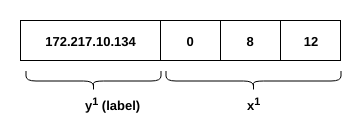
\includegraphics[width=0.70\textwidth]{training_example.png}
\caption{One training example} \label{fig:training_example}
\end{figure}


Before doing the clustering, we have to first determine the number clusters and centroids\footnote{Centroid is the vectors which is arithmetic mean of all the point in the cluster.} Deciding on the number of clusters is important, because randomly choosing the number of cluster will not be useful to have correct clustering. We will use the Elbow method to find the optimal number of clusters. The Elbow method check the percent of variance explained as function of the number of clusters. Following are the Eblow Diagrams for four samples.

\begin{figure}[H]
\centering
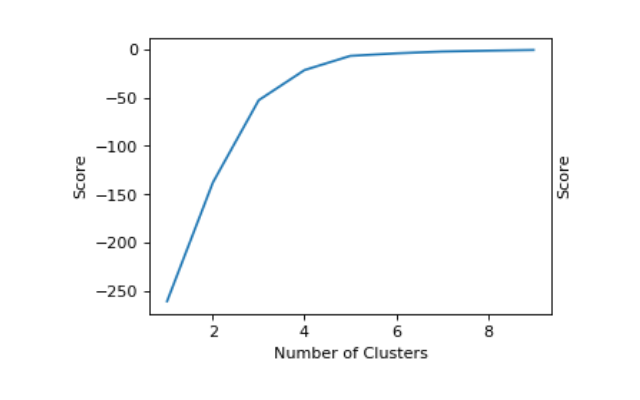
\includegraphics[width=0.90\textwidth]{elbow-method.png}
\caption{Elbow Method for cluster count detection} \label{fig:elbowmethod}
\end{figure}

Using the elbow method, variance for each cluster number is calculated and the cluster number which produces less variance for the next cluster number is selected as best choice for the give sample data.

To have correct clustering we first run the k-means algorithm to determine the central vectors called centroids. Clusters are represented by these centroids. As we have multiple `samples' (sample is the flow information) so we have cluster centroids for each sample. We will save all the centroids and then find the median of all the centroids removing the outliers so that we have good estimate of the centroids. This estimated centroids are used for clustering the samples in the future. Following is the example of centroid vector where rows represents cluster label and columns represent the feature.

\begin{table}[H]
\centering
  \begin{tabular}{ l | c  c  c }
    Cluster      & ICMP  & TCP  & UDP \\
    \hline
    0         &{-0.16815612}       &{-0.14928111}    &{-0.16948046} \\
    1         &{-0.18181818}       &{5.13527652}     &{5.68956244} \\
    2         &{5.08663322}        &{-0.27110845}    &{-0.099885} \\
    3         &{-0.18670401}       &{-0.18804342}    &{-0.018538} \\
  \end{tabular}
\caption{k-means cluster centroids} \label{table:centroids}
\end{table}

\begin{figure}[H]
\centering
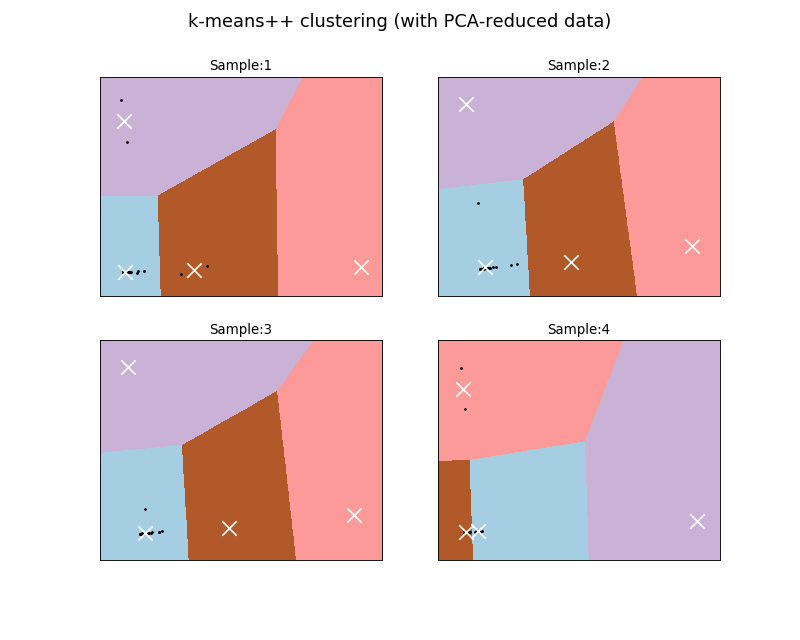
\includegraphics[width=0.90\textwidth]{kemans-clustering.png}
\caption{Clustering using k-means++ algorithm} \label{fig:k-means-clustering}
\end{figure}

To draw data points on 2 dimension space we had to reduce the 3 dimensional training example into 2 dimension without loosing much information. We have achieved this by using Principal-Component Analysis (PCA). PCA is a technique for taking a dataset consisting of a set of tuples representing points in the high-dimensional space and finding the directions along which the tuples line up best.\cite{pca}. We have used Scikit-learn PCA module for this purpose.

Using the centroids obtained in he previous step we ran k-means++ algorithm and then test it for accuracy. k-means++ algorithm gives label to an each training example. This label is the cluster number to which that training example has been assigned to. So the new labeled data look like following.

\begin{table}[H]
\centering
  \begin{tabular}{| l | c | c | c | c |}
    \hline
    {Destination IP Address}  &ICMP  &TCP &UDP  &Cluster \\
    \hline
    172.217.10.134  & 0     & 8     & 12  &1  \\ \hline
    65.19.96.252    & 5     & 0     & 192 &0  \\ \hline
    68.67.178.134   & 0     & 78    & 0   &2  \\ \hline
  \end{tabular}
\caption{Labeled Training Set (with cluster number)} \label{table:labeled-set}
\end{table}


We ran the k-means++ for both training and testing set and produce labels for both. We then checked how similar the test set clustering is with train set clustering i.e. we are checking if the IP address has the same cluster number assigned in both training and test data. For measuring this similarity Rand Index(RI)\cite{ri-index} is used. RI is a measure of how many percent does the test clustering matches with the trained model.

\hspace{4cm} $RI={\frac {TP+TN}{TP+FP+FN+TN}}$

where $TP, TN, TN$ and $FN$ are the number of true positives, true negatives, false positives and false negatives respectively.

We have observed that with more number of training sets RI index improves.

Because of the reason that the training sets contain the flow information for different IP on a router during window of 300 seconds, there is a very high possibility that the same destination IP address is captured in multiple training set. Our goal it to find out the correct cluster for the destination IP address, and to achieve this goal, we check all the cluster assignment for a given destination IP address and we select the cluster which has the highest occurring frequency among all the training sets. We also count the average number of packets going to a given IP address which will help us reduce the error in detecting anomaly. We will save this labeling information and cluster count information for each IP destination on the file system.

\begin{table}[H]
\centering
  \begin{tabular}{| l | c | c | c | c |}
    \hline
    {Destination IP Address}  &Cluster  &Packet Count \\
    \hline
    74.125.141.106  & 1     & 113  \\ \hline
    72.30.2.182     & 0     & 16   \\ \hline
    64.94.191.14    & 0     & 22   \\ \hline
  \end{tabular}
\caption{Learned information after clustering} \label{table:learned-clustering}
\end{table}

This information tell us the normal behavior of the packets traveling from the router to a given destination. As we have fixed the centroids for the clustering algorithm, every time in the future we should expect the IP address to be found in the same cluster if flow of packets for a given destination is as per the previous knowledge. If there is a DDoS attack on a any destination with flooding, then we can expect to see the destination IP address assigned to different cluster.

But from the experiments on different data sets it is found that the destination under attack is labeled with the same cluster number when it was not under attack. This happened because there is no other cluster it can assigned to, so it gets assigned to cluster whose centroid is nearest.

To avoid such situation, we will have to create the boundaries for the clusters. This scheme will make sure that the attack on the destination IP address will be detected even if the destination is assigned to the same cluster it was labeled in the past.

To create cluster boundaries we have used One Class SVM, a supervised machine learning algorithm. Compute and storage requirements of SVM increase rapidly with the number of training vectors, because SVM is a quadratic programming problem (QP). So the approach presented in the paper is more efficient because the number of cluster are limited and always be far less than the number of destination IP address. Training one class SVM on clusters will be far less process and memory intensive than training on massive number of IP address.

For example the number of clusters we have create in our analysis are 4 in number, while the number of IP addresses to which packets are flowing from our router are 268, which is more than 60 times the count of clusters we have created.

\subsubsection{Anomaly Detection using One Class Support-Vector Machine}

\paragraph{Support-Vector Machine:}

Support-Vector Machine is a supervised learning algorithm which tries to classify data. Classification is based on the label of the training set. Consider the training set $\{(x^{1},y^{1}),(x^{2},y^{2}), .., (x^{m},y^{m})\}$, where $x^{i} \in \mathbb{R}^d$ is the training example and $y^{i} \in \{-1, +1\}$ is the label which is the classification value for $x^{i}$,

SVM try to create non-linear separation boundary by projecting data points through a non-linear function $\phi$ to higher dimension space. The data points in space $I$ which can not be separated by a line are projected to the feature space $F$ where there can a hyperplane that separate data point of one class form another. If the hyperplane is projected back on original space $I$ then we get non-linear curve.\cite{svm}

\begin{figure}[H]
\centering
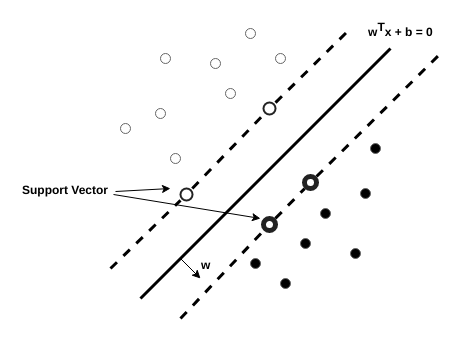
\includegraphics[scale=0.5]{SVM}
\caption{Linear Separation using Support Vector} \label{fig:SVM}
\end{figure}

The hyperplane is represented with the equation $w^{T}x + b = 0$, where $w \in F$ and $b \in R$. This hyperplane separates the training example labeled with $-1$ and $1$ into different classes. The position of the hyperplane is such that the distance from the closest point from each class to the hyperplane is same. To avoid the over-fitting, slack variables $\xi^{i}$ are introduced. Over-fitting happen because the learned hypothesis fit training examples so well that it fails to generalize the new examples. The constant $C > 0$ is the regularization parameter. If $C$ is chosen large, miss-classification of training examples can be avoided. If chosen small, then we may miss-classify few examples, but the margin will be large, so that most of the points will be far away from the decision boundary. The SVM optimization problem is stated as follows.\cite{svm} \cite{svm-ml}

\begin{center}
  ${min}_{w,b,\xi^i} \ \frac{||w||^2}{2} + C \sum_{i=1}^m \xi^i$ \\
  $\mbox{ subject to: }$ \\
  $y^i( w^T \phi(x^i) + b) \geq 1 - \xi^i \mbox{ for all } i = 1, \dots, m$ \\
  \hspace{3cm} $\xi^i \geq 0 \mbox{ for all } i = 1, \dots, m$ \\
\end{center}

If this minimization problem is solved using Lagrange multipliers then the classification function $f(x)$ can be stated as.

\begin{center}
$f(x)=sgn(\sum_{i=1}^m \alpha^i y^i K(x,x^i) \ + b)$
\end{center}

$\alpha^i$ here are the Lagrange multipliers and $x^i$ with $\alpha^i$ are called the Support Vectors.

The function $K(x,xi)=\phi(x)^T \phi(xi)$ is known as the kernel function. kernel function responsible for projecting data points to the hyperplane.

\paragraph{One Class Support-Vector Machine:}

One Class Support-Vector Machine (One Class SVM) is the extension of SVM which detect boundaries of the training set so that every new training example will be classifies as belong to training set or not. It separates all the training set data point from feature space $F$ and maximizes the distance of hyperplane from $F$. This creates a binary function which returns +1 for the training example that fits in the trained set region, otherwise it will return -1.

The minimization function of One Class SVM is slightly different than the SVM. \cite{svm}

\begin{center}
  ${min}_{w,\rho,\xi^i} \ \frac{||w||^2}{2} + \frac{1}{\nu n} \sum_{i=1}^m \xi^i - \rho$ \\
  $\mbox{ subject to: }$ \\
  $(w.\phi(x^i)) \geq \rho - \xi^i \mbox{ for all } i = 1, \dots, m$ \\
  \hspace{2cm} $\xi^i \geq 0 \mbox{ for all } i = 1, \dots, m$ \\
\end{center}

The new variable introduced $\nu$ in place of $C$ in previous SVM equation is used to set upper bound on outliers/anomalies and lower bound on the number of training examples.

We are using Scikit-learn's `OneClassSVM' library to train the model and create classifier for each cluster. The input vector to the classifier is the set of all the training examples belonging to same clusters. Thus, if we have four clusters then we will have four classifier. The input vector to the classier will be of the form shown in Table \ref{table:labeled-set}.

Following is the result of modeling on the training data sets. Each cluster has it own model.

\begin{figure}[H]
\centering
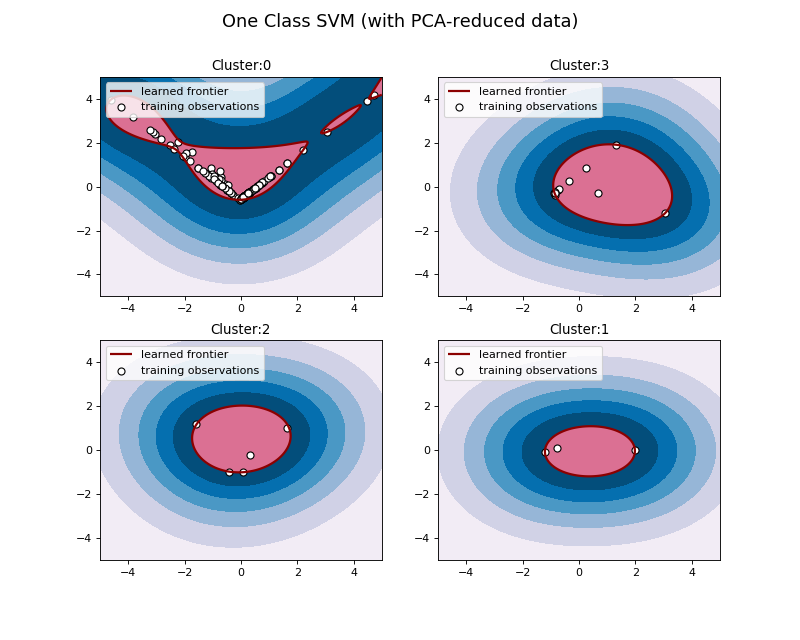
\includegraphics[width=0.80\textwidth]{one-class-SVM.png}
\caption{One Class SVM} \label{fig:one-class-SVM}
\end{figure}


\section{Detection}

By this stage, we have all the destination IP address, at the router, labeled with cluster and their count of average number of packets during the flow. Also we have classifier models for each of the cluster.

To detect the attack we capture the flow in the specified interval (e.g. 300 seconds, in which we have trained our models). We transformed the captured flow into a test set. The created test set is then clustered using already centroids which were calculated for the clustering of the training sets. Now we have each IP in the new test set labeled with the cluster number. If there is any destination IP address for which new cluster label does not match with the already known cluster label then that destination address added to the suspect list. If new label matches with the old then the feature vector for that destination address is passed to the cluster classifier to check it subsciption the cluster its found in. i.e. if an IP address is labeled with cluster number 0 then we use One Class SVM classifier for cluster number 0. If the output of the classifier is -1 then then that destination is added to the suspect list. For every destination from this compiled list, the number of packets observed is also recorded. If there is significant difference between the number of capture packet in the past and in the present then that destination is recorded as DDoS attack candidate because failing to found in the same cluster boundary it was in the past is a sign of the change in th behavior of the traffic for destination IP address on the router where this analysis is done.

Using this we have successfully detected attack on the destination IP address 92.168.0.7 in our modeled network.

Next task of the router then will be to communicate the change in the behavior of traffic observed at that router for a that destination. The destination address here could be a router or an application server. Destination system i.e. either router of the server will collect the information received. This information can be used by destination to know the nature of the attack.

\begin{figure}[H]
\centering
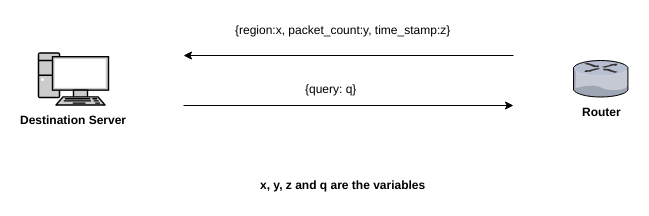
\includegraphics[scale=0.5]{router-network-communication}
\caption{Router Network Communication} \label{fig:router-network-communication}
\end{figure}

To Communicate the destination network about the change in behavior, router can use the existing ICMP protocol. ICMP protocol is used to provide feedback about problems in the communication environment. ICMP messages are sent in several situations:  for example 1) when a datagram cannot reach its destination. 2) when the gateway does not have the buffering capacity to forward a datagram. 3) when the gateway can direct the host to send traffic on a shorter route.\cite{icmp} Similarly we can use ICMP protocol to inform destination system about the change in the traffic. ICMP protocol has many unused type code (there can be 0-255 types but as of now only 0-41 are in use) available. We can create a new ICMP `type' to send DDoS detection information from the router to the destination system and then destination system can send mitigation instructions to the routers.

Depending on the type and the severity of the situation, the destination system can decide whether or not to inform router to block the traffic coming from that router. We will let this decision to be taken at the destination system. There can be different parameter based on which the destination system can decide blocking the flow. Many questions can be asked before making the decision, such as how many routers have reported the change in traffic?, Is the attack information coming from the region which never had traffic in the past?
\pagebreak
\section{Conclusion}
A novel way to identify and mitigate DDoS attack is discussed in this paper. With the advance of NVF(Network Virtual Functional) it is easy to push the learning algorithms to the routers allowing them to detect a DDoS attacks using machine learning algorithms. The DDoS detection and mitigation information can be communicated using existing ICMP protocol making system available to every one who want to use it. This approach has been tested with the small network so further experiments are needed to be performed on the larges networks.
\pagebreak

\singlespacing
\bibliographystyle{unsrt}   % Unsorted order
\bibliography{biblo}       % expects file "biblo.bib"

\end{document}
